\documentclass[xcolor=dvipsnames]{beamer}

\usepackage[utf8]{inputenc}
\usepackage[portuguese]{babel}
\usepackage[T1]{fontenc}
\usepackage{amsmath}
\usepackage{indentfirst}
\usepackage{amsfonts}
\usepackage{amssymb}
\usepackage{graphicx}
\usepackage{axodraw2}
\usepackage{subcaption}
\usepackage{appendixnumberbeamer}
\usepackage{multirow}

% Tikz com snakes
\usepackage{tikz}
\usetikzlibrary{snakes}

% Uso de uma fonte especial que eu acho bonite
\usepackage[math]{iwona}
%\usepackage{fourier}

\usetikzlibrary{3d}
\DeclareMathOperator*{\sen}{sen}
\renewcommand{\vec}{\mathbf}

\usetheme{Madrid}

\definecolor{azulUFPel}{rgb}{0.0, 0.25, 0.55}

\usecolortheme[named=azulUFPel]{structure}
\usefonttheme{serif}

% Uns trecos que eu fiz pra ficar mais ao meu gosto estético
\setbeamertemplate{itemize item}[triangle]
\setbeamertemplate{itemize subitem}[square]
\setbeamertemplate{enumerate item}[square]
\setbeamertemplate{navigation symbols}{}
\setbeamertemplate{section in toc}[circle]
\title{Método dos Fótons Equivalentes}
\subtitle{Revisão e Aplicações}
\author[A. A. S. Pacheco]{
	Alfredo Achterberg S. Pacheco\\
	{\footnotesize Orientador: Prof.  Dr. Werner Krambeck Sauter}\\
	{\scriptsize Defesa da Proposta de Trabalho de Conclusão de Curso}
}
\institute[IFM - UFPel]{
	Curso de Bacharelado em Física - Universidade Federal de Pelotas
}
\date[25 de set., 2023]{25 de Setembro, 2023}
\titlegraphic{
	
\includegraphics[height=1.5cm]{./logos/logoUFPEL.png}
	\hspace{1cm}
	
\includegraphics[height=1.5cm]{./logos/logoFISICA.jpg}
}
%\logo{
\includegraphics[width=0.15\textwidth]{logoUFPel.png}}

\begin{document}

\frame{\titlepage}

\begin{frame}
\frametitle{Estrutura da Apresentação}
\tableofcontents
\end{frame}

\section{Introdução e Contextualização}

\begin{frame}
	\frametitle{Introdução e Contextualização}
	\begin{columns}
	\column{0.5\textwidth}	
		\begin{figure}
			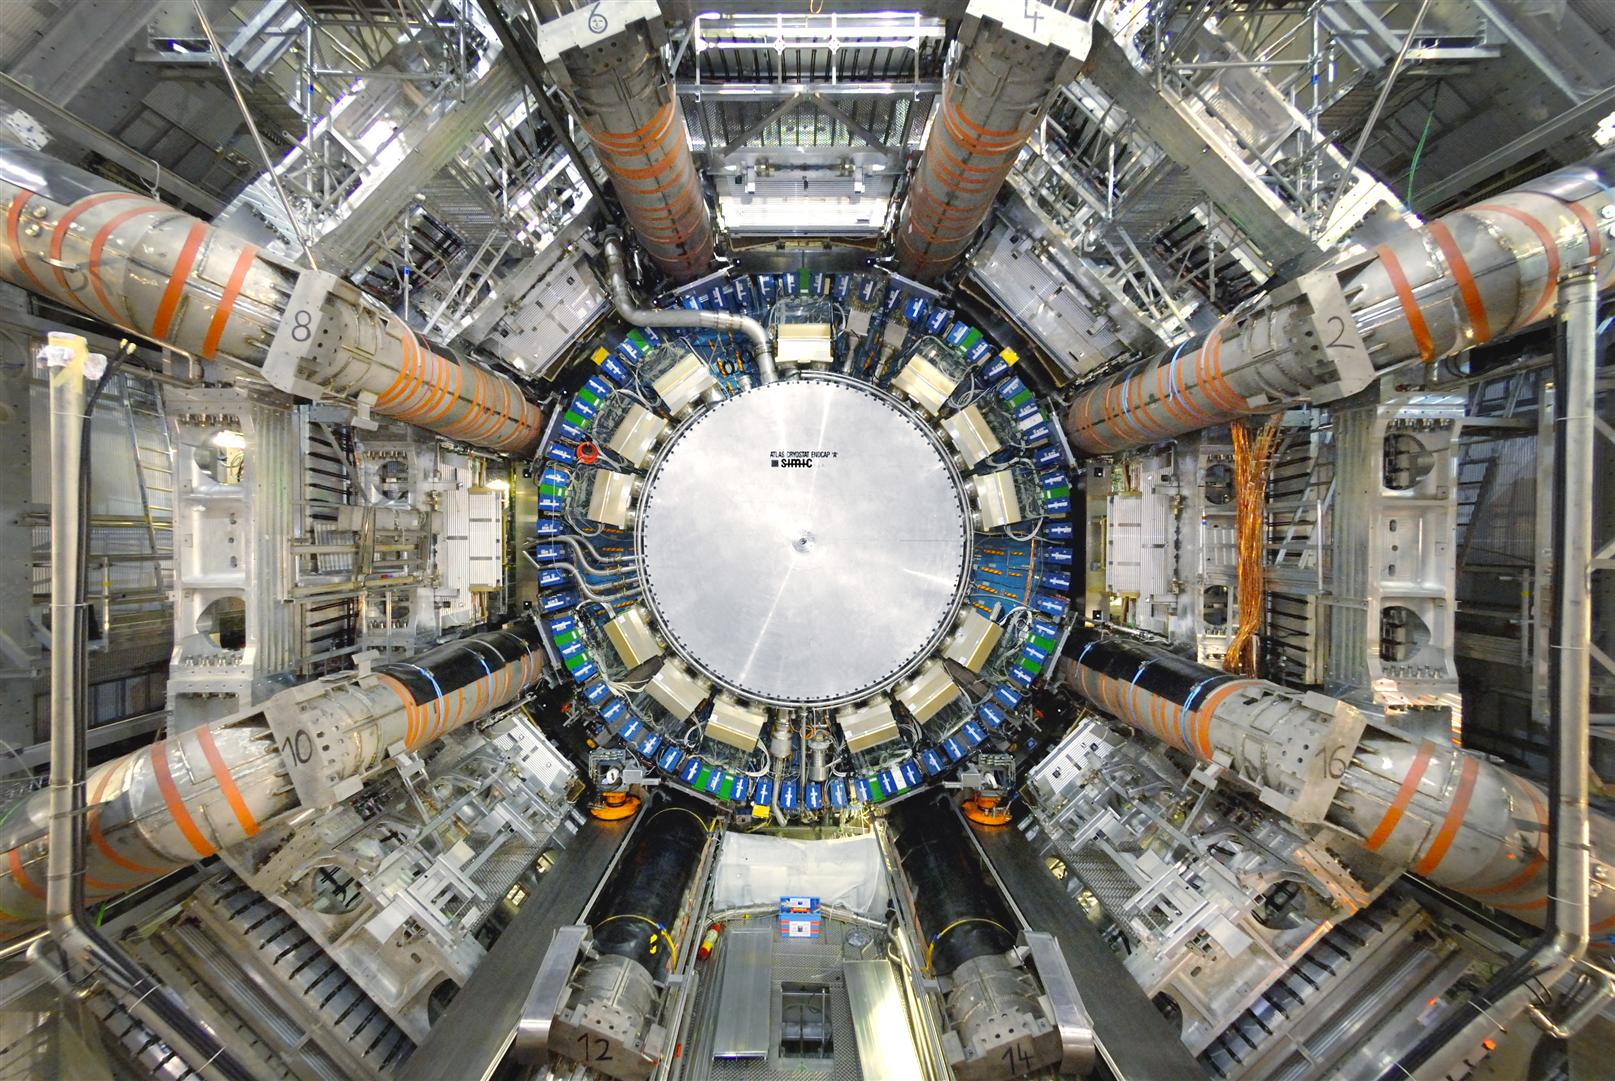
\includegraphics[width=\columnwidth]{./figs/atlan_normal.jpg}
			\caption{Foto do detector ATLAS do LHC. {\scriptsize Créditos:
			[\url{https://home.web.cern.ch/science/experiments/atlas}]}}
		\end{figure}
	
	\column{0.5\textwidth}
		Colisões de partículas constituem o método experimental mais utilizado
		atualmente para o entendimento da estrutura fundamental da matéria e de
		teste para novos modelos físicos.
	\end{columns}
\end{frame}

\begin{frame}
	\frametitle{Introdução e Contextualização}
	Estudos desse tipo de processo tem longa história na física.
	\begin{itemize}
		\item O trabalho de decréscimo de velocidade de partículas $\alpha$ e
			$\beta$ em meios materiais por N. Bohr, realizado em 1913;
		\item este propôs que a interação de partículas
			carregadas pode ser entendida pelo fenômeno eletromagnético de
			dispersão (uma analogia);
		\item em 1924, E. Fermi propôs que os campos de uma partícula carregada
			podem ser aproximados como pulsos de onda ou \textit{fluxos de
			fótons virtuais.}
	\end{itemize}
\end{frame}

\begin{frame}
	\frametitle{Introdução e Contextualização}
	\begin{columns}
	\column{0.5\textwidth}
		Disso, E. J. Williams, em 1933, propôs a generalização relativística do
		que seria o método dos fótons equivalentes.
		\begin{itemize}
			\item consiste em obter o número de fótons virtuais a partir da 
				transformada de Fourier dos campos $\vec{E}$ e $\vec{B}$;
			\item este consiste de uma aproximação \textit{semi-clássica}.
		\end{itemize}

	\column{0.5\textwidth}
		\begin{figure}
			\begin{tikzpicture}[thick]
	\draw(-2,2) ellipse (0.15 and 0.75);
	\draw(0,0) ellipse (0.15 and 0.75);
	\node[left] (z1) at (-2.15,2) {$Z_1e$};
	\node[right] (z2) at (0.15,0) {$Z_2 e$};

	\draw[->](-2,2.75) -- (-2,3.75);
	\draw[->, rotate around={15:(-2,2.75)}](-2,2.75) -- (-2,3.75);
	\draw[->, rotate around={-15:(-2,2.75)}](-2,2.75) -- (-2,3.75)
		node[right]{$\vec{E}$};

	\draw[->](-2,1.25) -- (-2,0.25);
	\draw[->, rotate around={15:(-2,1.25)}](-2,1.25) -- (-2,0.25);
	\draw[->, rotate around={-15:(-2,1.25)}](-2,1.25) -- (-2,0.25);

	\draw[->](0,0.75) -- (0,1.75);
	\draw[->, rotate around={15:(0,0.75)}](0,0.75) -- (0,1.75);
	\draw[thick, ->, rotate around={-15:(0,0.75)}](0,0.75) -- (0,1.75);

	\draw[->](0,-0.75) -- (0,-1.75);
	\draw[->, rotate around={15:(0,-0.75)}](0,-0.75) -- (0,-1.75);
	\draw[->, rotate around={-15:(0,-0.75)}](0,-0.75) -- (0,-1.75);

	\draw[->](-1.85,2) -- (-1,2);
	\draw[->](-0.15,0) -- (-1.15,0) node[below]{$v \approx c$};
\end{tikzpicture}


			\caption{Esquema representando os campos relativísticos de dois íons
			$Z_1$ e $Z_2$. Adaptado de \cite{bertulani2005}.}
		\end{figure}
	\end{columns}
\end{frame}

\begin{frame}
	\frametitle{Introdução e Contextualização}
	\begin{itemize}
		\item Há motivação para o estudo do método nas áreas de interação
			nuclear e de partículas;
		\item focaremos nas colisões ultraperiféricas de íons;
		\item são colisões com maior distância (parâmetro de impacto) e com
			interação dominantemente eletromagnética;
		\item por conta disso, também há menos multiplicidade nos estados
			finais e os resultados experimentais são mais facilmente tratados;
		\item fenômenos de interesse incluem a produção de pares de partículas
			a partir de colisões de fótons.
	\end{itemize}
\end{frame}

\section{Objetivos do Trabalho}
\begin{frame}
	\frametitle{Objetivos do Trabalho}
	Para a realização do trabalho propomos uma revisão bibliográfica com cálculo
	analítico e computacional de quantidades de interesse dos processos de
	colisão. Para isso, temos os seguintes objetivos específicos:
	\begin{enumerate}
		\item realizar a revisão bibliográfica do método;
		\item realizar o cálculo do fator de forma para o fator de forma
			para diferentes distribuições de carga;
		\item deduzir o número de fótons equivalentes para diferentes
			distribuições de carga;
		\item realizar um estudo mais aprofundado sobre o fenômeno de
			fotoprodução de pares de partícula-antipartícula;
		\item obter as curvas teóricas para as seções de choque de diferentes
			processos de colisão e compará-las com as curvas experimentais.
	\end{enumerate}

\end{frame}

\section{Seção de Choque Diferencial e Total}
\begin{frame}
	\frametitle{Seção de Choque Diferencial e Total}
	O problema de interesse do método é o de colisão de partículas carregadas.
	A quantidade de interesse em colisões é a seção de choque.
	\begin{figure}[h]
		\centering
		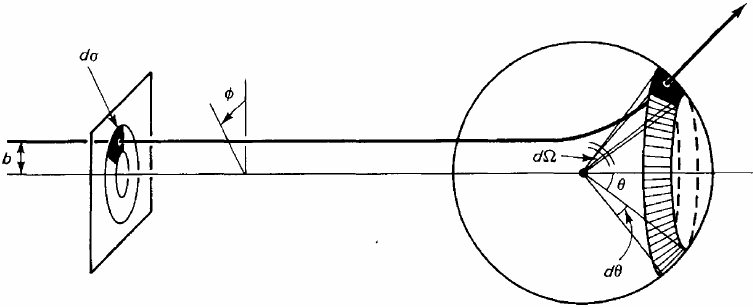
\includegraphics[width=0.8\textwidth]{./figs/cross_section.jpeg}
		\label{fig_cross_section}
		\caption{Partícula adentrando a região de espalhamento por uma
		seção de área $d\sigma$ e  sendo espalhada em um ângulo sólido
		$d\Omega$. Retirado de \cite{griffiths_particle}.}
	\end{figure}
\end{frame}

\begin{frame}
	\frametitle{Seção de Choque Diferencial e Total}
	Da figura temos as diferenciais,
	\begin{gather}
		d\sigma = |b\, db\, d\phi|,\\
		d\Omega = |\sen \theta \, d\theta \, d\phi|, \\ \Rightarrow
		\frac{d\sigma}{d\Omega} = \bigg| \frac{b}{\sen \theta}
		\frac{db}{d\theta} \bigg|. \label{diff_cross_section}
	\end{gather}

	A seção de choque total vem pela integral sobre $\Omega$,
	\begin{equation}
		\sigma = \int \frac{d\sigma}{d\Omega} \sen \theta \, d\theta \, d\phi .
	\end{equation}
	\begin{block}{Isto para uma partícula incidente individual!}
		Estamos levando em conta uma partícula individual. Se quisermos tratar
		um feixe de partículas, vamos precisar definir a \textit{luminosidade}.
	\end{block}

\end{frame}

\begin{frame}
	\frametitle{Seção de Choque Diferencial e Total}
	\begin{block}{Luminosidade}
		Para um feixe de $N$ partículas com mesma energia atravessando a área
		$d\sigma$, a luminosidade $\mathcal{L}$ é definida como a quantidade
		de partículas que atravessam a região de espalhamento por unidade de
		área por unidade de tempo.
	\end{block}
	Disso, reescrevemos a seção de choque para um feixe de múltiplas partículas,
	\begin{gather}
		dN = \mathcal{L} d\sigma, \\
		\Rightarrow \frac{d\sigma}{d\Omega} = \frac{1}{\mathcal{L}}
		\frac{dN}{d\Omega}.
	\end{gather}
\end{frame}

\section{Demonstração do Método}
\begin{frame}
	\frametitle{Demonstração do Método para Carga Pontual}
	Inicialmente consideramos uma carga em movimento como abaixo.\footnote{A
	partir daqui usaremos unidades naturais ($\hslash = c = 1$).}
	\begin{figure}
	\begin{tikzpicture}[thick, scale=0.65]
	% A caceta dos eixos...
		\draw[-] (0,0) --  (13,0)node[right]{$x_1$};
		\draw[-] (0,0) -- (0,4) node[above]{$x_2$};
		\draw[-] (0,0) -- (0,0,3) node[below left]{$x_3$};
		\draw[-] (5,0.4) -- (13.5,0.4) node[right]{$x'_1$};
		\draw[-] (5,0.4) -- (5,4) node[above]{$x' _2$};
		\draw[-] (5,0.4) -- (5,0.2,3) node[below left]{$x'_3$};

	% A caceta dos desenhos que importam
		\filldraw (5,0.4) circle(3pt) node[above right] {$q$};
		\filldraw (0,3) circle(3pt) node[above right] {$P$};
		\draw (0,3) -- node[above]{$r$} (5,0.4);
		\draw[|-|,dashed] (-0.3,0) -- node[fill=white,left]{$b$} (-0.3,3);
		\draw[->,ultra thick] (5,0.4) -- (7,0.4) node[above]{$\vec{v}$};
\end{tikzpicture}


	\caption{Carga $q$ em movimento com velocidade $\vec{v}$ passando por um
		ponto de observação $P$ com parâmetro de impacto $b$ e distância $r$.
		Referencial $\Sigma$ é solidário ao ponto $P$ e $\Sigma '$ é solidário
		à carga pontual $q$. Adaptado de \cite{jackson3}.}
	\end{figure}
\end{frame}

\begin{frame}
	\frametitle{Demonstração do Método para Carga Pontual}
	Os campos $\vec{E}$ e $\vec{B}$ são escritos em forma explicitamente
	covariante usando o tensor eletromagnético,
	\begin{equation}
		F^{\mu \nu} = \begin{pmatrix}
			0 & -E_1 & -E_2 & -E_3 \\
			E_1 & 0 & -B_3 & B_2 \\
			E_2 & B_3 & 0 & -B_1 \\
			E_3 & -B_2 & B_1 & 0
		\end{pmatrix}.
	\end{equation}
	A tranformada de Lorentz das componentes deste tensor é dada por,
	\begin{equation}
		{F'}^{\mu \nu} = \frac{\partial {x'}^\mu}{\partial x^ \alpha}
		\frac{\partial {x'}^\nu}{\partial x^\beta}F^{\alpha \beta} = \Lambda
		^\mu _\alpha \Lambda ^\nu _\beta F^{\alpha \beta}.
	\end{equation}
\end{frame}

\begin{frame}
	\frametitle{Demonstração do Método para Carga Pontual}
	$\Lambda^\mu _\nu$ são as componentes da matriz de transformação de Lorentz,
	dada, para o nosso caso, como,
	\begin{equation}
		(\Lambda ^\mu _\nu) = \begin{pmatrix}
			\gamma & -\gamma \beta & 0 & 0 \\
			-\gamma \beta & \gamma & 0 & 0 \\
			0 & 0 & 1 & 0 \\
			0 & 0 & 0 & 1
		\end{pmatrix},
	\end{equation}
	sendo $\displaystyle \gamma = \frac{1}{\sqrt{1-\beta ^2}}$ e $\beta = v/c$
	os parâmetros relativísticos da partícula. O cálculo dos termos não nulos
	leva a,
	\begin{equation}
		\label{eq_field_trans}
		\begin{cases}
		E_1' = E_1 \\
		E_2' = \gamma (E_2 - \beta B_3) \\
		E_3' = \gamma (E_3 + \beta B_2) \\
		\end{cases} \qquad
		\begin{cases}
		B_1 ' = B_1 \\
		B_2 ' = \gamma (B_2 + \beta E_3) \\
		B_3' = \gamma(B_3 - \beta E_2)
		\end{cases}.
	\end{equation}
\end{frame}

\begin{frame}
	\frametitle{Demonstração do Método para Carga Pontual}
	Escrevendo os campos nas \textit{coordenadas} de $\Sigma$ e depois
	aplicando a transformada de Lorentz temos os campos no \textit{referencial}
	$\Sigma$,
	\begin{gather}
		E_1 (t) = -\frac{q\gamma vt}{(b^2 + \gamma ^2 v^2t^2)^{3/2}}
			\label{eq_field1},\\
		E_2 (t) = \frac{q\gamma b}{(b^2 + \gamma ^2 v^2 t
			^2)^{3/2}}\label{eq_field2},\\ 
		B_3 (t) = \beta E_2(t) \label{eq_field3}.
	\end{gather}
	\begin{block}{Aproximamos estes campos como pulsos de onda.}
		Analisando esses campos podemos notar que $E_2$ e $B_3$ formam um pulso
		de onda na direção $x_1$. Ainda assim, a interação do campo $E_1$ pode
		ser analisada como um pulso de onda pela inserção de um campo magnético
		artificial como aproximação.
	\end{block}
\end{frame}

\begin{frame}
	\frametitle{Demonstração do Método para Carga Pontual}
	\begin{figure}
		\begin{subfigure}[b]{0.4\textwidth}
			\centering
			\begin{tikzpicture}[thick]
	\draw[-] (0,0) --  (3,0)node[right]{$x_1$};
	\draw[-] (0,0) -- (0,2.5) node[above]{$x_2$};
	\draw[-] (0,0) -- (0,0,1) node[below left]{$x_3$};

	\draw[->, blue] (2,1.5) -- (2,3.5) node[left]{$E_2$};
	\draw[->, blue] (2,1.5) -- (3.5,1.5) node[right]{$E_1$};
	\draw[->, blue] (2,1.5) -- (2,1.5,2) node[below]{$B_3$};

	\filldraw (2,1.5) circle(3pt) node[above left] {$P$};
\end{tikzpicture}

			\caption{Campos observados no referencial do ponto $P$.}
		\end{subfigure}
		\hspace{1cm}
		\begin{subfigure}[b]{0.4\textwidth}
			\centering
			\begin{tikzpicture}[thick]
	\draw[-](-1,0) -- (1,0) node[right]{$x_1$};
	\draw[-](0,0) -- (0,2.5) node[above]{$x_2$};

	\filldraw (0,1.5) circle(3pt) node[above right]{$P$};

	\draw[
		->,
		snake = coil,
		segment aspect=0,
		segment length=5pt,
		segment amplitude=5pt,
		line after snake=2pt,
		blue
	] (0,0) -- (0,1) node[left]{$P_2$};
	\draw[
		->,
		snake = coil,
		segment aspect=0,
		segment length=5pt,
		segment amplitude=5pt,
		line after snake=2pt,
		blue
	] (-1.5,1.5) -- (-0.5,1.5) node[above]{$P_1$};
\end{tikzpicture}

			\caption{Pulsos aproximados $P_1$ e $P_2$ atingindo $P$.}
		\end{subfigure}
		\caption{Aproximação chave do método dos fótons virtuais é a de
		substituir os campos elétrico e magnético por pulsos de radiação
		equivalentes. Ambas as figuras adaptadas de \cite{caruso_quanta}.}
	\end{figure}
\end{frame}

\begin{frame}
	\frametitle{Demonstração do Método para Carga Pontual}
	Com isso, iremos calcular agora os espectros de frequência\footnote{A
	energia por unidade de frequência e área de um pulso}, para ambos os
	pulsos. Estes o são
	\begin{gather}
		I_1(\omega , b) = \frac{1}{2\pi} |E_2 (\omega) |^2 ,\\
		I_2 (\omega , b) = \frac{1}{2\pi} |E_1 (\omega)|^2,
	\end{gather}
	em que 
	\begin{equation}
		E_{1,2} (\omega) = \frac{1}{\sqrt{2\pi}} \int _{-\infty}^{+\infty}
		dt \; E _{1,2} (t) e^{i\omega t},
	\end{equation}
	é a transformada de Fourier da parte elétrica dos pulsos.
\end{frame}

\begin{frame}
	\frametitle{Demonstração do Método para Carga Pontual}
	O cálculo da integral para os dois campos leva ao seguinte resultado,
	\begin{gather}
		I_1 (\omega , b) = \frac{1}{\pi ^2} \frac{q^2}{ \beta ^2 b^2}  
		\xi ^2 K_1 ^2 \left( \xi \right), \\
		I_2 (\omega , b) = \frac{1}{\pi ^2} \frac{q^2}{\beta ^2 b^2 }
		\frac{1}{\gamma ^2} \xi^2 K_0 ^2 \left( \xi \right),
	\end{gather}
	onde $\displaystyle \xi \equiv \frac {\omega b}{\gamma v}$ e as
	funções $K_1$ e $K_0$ são as funções modificadas de Bessel.
\end{frame}

\begin{frame}
	\frametitle{Demonstração do Método para Carga Pontual}
	A partir disso, o número de fótons equivalentes pode ser obtido pelo
	espectro de frequência como,
	\begin{equation}
		\begin{split}
		N(\omega , b) &= \frac{1}{\omega} \left[ I_1 (\omega , b) + I_2(\omega
			, b) \right]\\
			&= \frac{1}{\pi ^2} \frac{q^2} {\beta ^2 b^2}
			\frac{1}{\omega ^2} \xi ^2 \left[K_1^2 (\xi ) + \frac{1}{\gamma ^2}
			K_0 ^2 (\xi ) \right]. \label{eq_EP-SPEC}
		\end{split}
	\end{equation}
	\begin{block}{Este pode ser simplificado:}
		Por conta do fator $\gamma ^{-2}$, para velocidades relativísticas
		altas o termo com $K_0$ contribui pouco para o fluxo de fótons e
		podemos escrever,
		\begin{equation}
			N(\omega , b) = \frac{1}{\pi ^2} \frac{q^2} {\beta ^2 b^2}
			\frac{1}{\omega ^2} \xi ^2 K_1 ^2 (\xi).
		\end{equation}
	\end{block}
\end{frame}

\begin{frame}
	\frametitle{Demonstração do Método para Carga Pontual}
	O número de fótons total é dado pela integral de $N(\omega , b)$ sobre os
	parâmetros de impacto,
	\begin{multline}
		n(\omega) = \int _{b_{\text{min}}}^\infty db\; bN(\omega , b)  
		= \frac{1}{\pi} \frac{2q^2}{\beta ^2} \frac{1}{\omega} \biggl\{ \xi
		_\text{min} K_0 \left( \xi \right) K_1 \left( \xi _\text{min} \right) 
		\\
		-\frac{\beta ^2}{2} \xi _\text{min} ^2 \left[ K_1 ^2 \left( \xi
		_\text{min} \right) - K_0 ^2 \left( \xi _\text{min} \right) \right]
		\biggr\}. \label{eq_EPT}
	\end{multline}
\end{frame}

\section{Sobre o Fator de Forma}
\begin{frame}
	\frametitle{Sobre o Fator de Forma}
	Para o caso da partícula incidente não ser pontual é introduzido o
	\textit{fator de forma} $F(|\vec{q}|)$. Assim, o $N(\omega , b)$ fica
	escrito como,
	\begin{equation}
		N(\omega , b) = \frac{1}{\pi ^2} \frac{Z^2 \alpha}{\beta ^2 \omega b^2}
		\Bigg| \int du \; u^2 J_1 (u) \frac{F[(u^2 + \xi ^2)/b^2]}{u^2 + \xi ^2}
		\Bigg|^2. \label{eq_EP-SPEC-F}
	\end{equation}
	O fator de forma $F(|\vec{q}|)$ é a transformada de Fourier da distribuição
	de carga $f(\vec{r})$. $\vec{q}$ aqui é a tranferência de momento na
	colisão.
\end{frame}

\begin{frame}
	\frametitle{Sobre o Fator de Forma}
	\begin{itemize}
		\item A maior parte das distribuições de carga são esfericamente
			simétricas.
	\end{itemize}
	{\footnotesize \renewcommand{\arraystretch}{3}
	\begin{table}
		\begin{tabular}{|c|c|}
	$f(r)$ & $F(|\vec{q}|)$ \\
	\hline
	 $\delta (r) / 4 \pi$ & 1 \\
	$\displaystyle \frac{a^3}{8\pi} e^{-ar}$ &
	$\displaystyle \left(\frac{1 + |\vec{q}|^2}{a^2}\right) ^{-2}$\\
	$ \left( a^2 / 2\pi \right)^{3/2} e
	^{-a^2 r^2 / 2}$ & $e^{|\vec{q}|^2 / 2a^2 }$ \\
	 $\displaystyle \begin{cases}
		3/4\pi R^3, & r \leq R \\
		0, & r > R
	\end{cases}$ & $ \displaystyle \frac{3(\sen \alpha - \alpha \cos
	\alpha)}{\alpha}$, $\alpha = |\vec{q}| R$ 
	\\
\end{tabular}


		\caption{Fatores de forma disponíveis para diferentes distribuições de
		carga esfericamente simétricas. Tabela retirada de \cite{povh6ed}.}
	\end{table}
	}
\end{frame}


\section{Colisões Ultraperiféricas}
\begin{frame}
	\frametitle{Colisões Ultraperiféricas}
	\begin{itemize}
		\item Possuem alto parâmetro de impacto $b$.
		\item A interação é predominantemente eletromagnética.
		\item Estados finais tem baixa multiplicidade $\rightarrow$ dados
			experimentais mais limpos!
		\item Fenômenos de interesse ocorrem como a produção de partículas por
			colisão de fótons.
	\end{itemize}
\end{frame}

\begin{frame}
	\frametitle{Colisões Ultraperiféricas}
	\begin{figure}
		\begin{subfigure}[b]{0.45\textwidth}
			\centering
			\begin{axopicture}(100,100)
	\Line[arrow](0,0)(50,25)
	\Line[arrow](50,25)(100,0)
	\Line[arrow](0,100)(50,75) 
	\Line[arrow](50,75)(100,100)
	\Photon(50,25)(50,75){3}{7}
	\Line[arrow,double](50,25)(100,25)
	\Vertex(50,25){4}
	\Text(10,5)[rb]{$Z_2$}
	\Text(10,95)[rt]{$Z_1$}
	%\Text(190,5)[lb]{$Z_2$}
	%\Text(190,95)[lt]{$Z_1$}
	\Text(100,30)[rb]{$X$}
	\Text(55,50)[l]{$\gamma$}
\end{axopicture}


			\caption{Processo de excitação do íon $Z_2$ pelo fóton $\gamma$ e
			produção do estado final $X$.}
		\end{subfigure}
		\hspace{0.25cm}
		\begin{subfigure}[b]{0.45\textwidth}
			\centering
			\begin{axopicture}(100,100)
	\Line[arrow](0,0)(50,25)
	\Line[arrow](50,25)(100,0)
	\Line[arrow](0,100)(50,75)
	\Line[arrow](50,75)(100,100)
	\Photon(50,25)(50,75){3}{7}
	\Line[arrow,double](50,50)(100,50)
	\BCirc(50,50){7}
	\Text(10,5)[rb]{$Z_2$}
	\Text(10,95)[rt]{$Z_1$}
	\Text(100,55)[rb]{$X$}
	\Text(45,35)[r]{$\gamma$}
	\Text(45,65)[r]{$\gamma$}
\end{axopicture}


			\caption{Processo de produção do estado $X$ por colisão dos fótons
			$\gamma$.}
		\end{subfigure}
		\caption{Fenômenos de fotoprodução de estados $X$. Ambas as figuras retiradas
		de \cite{bertulani2005}.}
	\end{figure}
\end{frame}

\begin{frame}
	\frametitle{Colisões Ultraperiféricas}
	\begin{block}{As seções de choque são calculadas com $n(\omega)$}
		As seções de choque dos processos são obtidos com o número de fótons
		equivalentes. Para os processos de excitação e colisão de fótons temos,
		respectivamente,
		\begin{gather}
			\sigma _X = \int d\omega \; \frac{n(\omega)}{\omega} \sigma _X
			^\gamma (\omega) \\
			\sigma _{Z_1 Z_2 \rightarrow X} = \int d\omega _1 d\omega _2 \;
			\frac{n(\omega _1)}{\omega _1} \frac{n(\omega _2)}{\omega _2}
			\sigma_{\gamma \gamma \rightarrow X}(\omega _1, \omega _2),
		\end{gather}
		onde $\sigma _X ^\gamma$ é a seção de choque fotonuclear e $\sigma
		_{\gamma \gamma \rightarrow X}$ é a seção de choque fóton-fóton.
	\end{block}
\end{frame}

\begin{frame}
	\frametitle{Colisões Ultraperiféricas}
	\begin{itemize}
		\item Energia (a frequência $\omega$) e parâmetro de impacto mínimo
			são relacionados aos parâmetros dos experimentos de colisão;
		\item Destacamos a luminosidade e a energia máxima de colisão
			$\displaystyle \omega _\text{max} \sim \frac{\gamma v}{b}$;
		\item Estes são relacionados com a quantidade de íons por feixe e a
			energia máxima com que estes colidem.
	\end{itemize}
\end{frame}

\begin{frame}
	\frametitle{Colisões Ultraperiféricas}
	\begin{table}
		\begin{tabular}{lccc}
	\hline
	Íons & Acelerador & $\omega _\text{max}$ & $\mathcal{L}$
		[$10^{30}$cm$^{-2}$s$^{-1}$]\\
	\hline
	\multirow{3}{4em}{$e^+ \; e^-$} & VEPP (Novosibirsk) & 6,0 GeV & 20
	\\
	& BEPC-II (China) & 1,89 GeV & 1000 \\
	& CESR-C (Cornwell) & 6,0 GeV & 76 \\
	$p \; p$ & LHC (CERN) & 6,5 TeV & 2,11 $\cdot 10^{4}$ \\
	$p \; \bar{p}$ & TEVATRON (Fermilab) & 0,980 TeV & 431 \\
	$Au \; Au$ & RHIC (Brookhaven) & 0,1 TeV & 8,7 \\
	$p \; Au$ & RHIC & 0,1 TeV & 450 \\
	$Xe \; Xe$ & LHC & 2,72 TeV & 0,4 \\
	\hline
\end{tabular}


		\caption{Parâmetros de experimentos de alguns colisores. Tabela baseada
		em \cite{Workman2022ynf}.}
	\end{table}
\end{frame}

\section{Metodologia}
\begin{frame}
	\frametitle{Metodologia}
	\begin{itemize}
		\item Revisão mais aprofundada da literatura sobre os temas discutidos;
		\item refazer os cálculos analíticos para as quantidades de interesse
			nos casos em que for possível:
			\begin{itemize}
				\item Fatores de forma $F(|\vec{q}|)$;
				\item números de fótons $N(\omega ,b)$ e $n(\omega)$;
				\item seções de choque $\sigma$.
			\end{itemize}
		\item obter as curvas teóricas e realizar cálculos computacionais com
			auxílio da biblioteca GSL (\textit{Gnu Scientific Library}) para
			C++.
	\end{itemize}
\end{frame}

\section{Cronograma}
\begin{frame}
	\frametitle{Cronograma}
	{ \small
	\begin{table}
		\begin{tabular}{lccccc}
	\hline
	& Mês 1 & Mês 2 & Mês 3 & Mês 4 & Mês 5\\
	\hline \hline
	1) Revisão bibliográfica & $\times$ & $\times$ & $\times$ &
	$\times$ & \\
	2) Dedução dos $F(|\vec{q}|)$ & $\times$
		 & $\times$ & $\times$ & & \\
	3) Cálculo de $N(\omega, b)$ e $n(\omega)$ & & $\times$ & $\times$
	& $\times$ & \\
	4) Obtenção das $\sigma$ & & $\times$ &
	$\times$ & $\times$ & \\
	5) Redação do TCC & & & $\times$ & $\times$ & $\times$ \\
	6) Defesa do TCC & & & & & $\times$ \\
	\hline
\end{tabular}


		\caption{Cronograma a ser seguido na execução do projeto.}
	\end{table}
	}
\end{frame}

\begin{frame}[allowframebreaks]
	\frametitle{Referências}
	\bibliographystyle{apalike}
	\bibliography{./../docs/bibtex.bib}  
\end{frame}

\begin{frame}
	\frametitle{Agradecimentos}
	\begin{center}
		
\includegraphics[width=2cm]{./logos/logoFNDE.png}
		\hspace{2cm}
		
\includegraphics[width=2cm]{./logos/logoPET.png}
	\end{center}
\end{frame}

\appendix
\begin{frame}
	\frametitle{Dedução da Transformada de Lorentz para os Campos}
	Sendo os campos elétrico e magnético escritos em termos dos potenciais,
	\begin{gather}
		\vec{E} = - \nabla \Phi - \frac{\partial \vec{A}}{\partial t}, \\
		\vec{B} = \nabla \times \vec{A},
	\end{gather}
	estes são escritos em forma explicitamente covariante usando o tensor
	eletromagnético,
	\begin{equation}
		F^{\mu \nu} = \begin{pmatrix}
			0 & -E_1 & -E_2 & -E_3 \\
			E_1 & 0 & -B_3 & B_2 \\
			E_2 & B_3 & 0 & -B_1 \\
			E_3 & -B_2 & B_1 & 0
		\end{pmatrix}.
	\end{equation}
\end{frame}

\begin{frame}
	\frametitle{Como escrevemos os Campos nas Coordenadas de $\Sigma$}
	\begin{columns}

	\column{0.5\textwidth}
		Os campos como percebidos em $P$, no referencial $\Sigma '$ tem a forma
		\begin{equation}
			E_1 ' = -\frac{qvt'}{{r'} ^3}, \qquad E_2 ' = \frac{qb}{{r'}^3}.
		\end{equation}
		Escrevemos nas \textit{coordenadas} de $\Sigma$ usando,
		\begin{gather}
			t' = \gamma t, \\
			\begin{split}
				r ' &= \sqrt{b^2 + (v t')^2} \\
					&= \sqrt{b^2 + v^2 \gamma ^2 t^2}.
			\end{split}
		\end{gather}

	\column{0.5\textwidth}
		Assim
		\begin{gather}
			E _1 '= - \frac{q\gamma vt}{(b^2 + \gamma ^2 v^2 t^2)^{3/2}},\\
			E _2 '= \frac{qb}{(b^2 + \gamma ^2 v^2 t^2)^{3/2}},
		\end{gather}
		para os quais devemos aplicar a transformação de Lorentz.
	\end{columns}
\end{frame}


\end{document}
